\section{Ergebnisse}

\begin{flushleft}
In \hl{Abb. x} ist der Ausgangsstrom geplotet gegen die \hl{Zeit} zu sehen. Der erste Graph ist eine darstellung der Daten ohne Frequenz filter, der zweite mit. Der Frequenzfilter ist für die visualisierung notwendig, da der Wandler eine Standardabweichung von mehreren Milliampere besitzt. Für weiteres wird nun immer eine Visualisierung mit Frequenzfilter verwendet insofern nicht anders genannt. Es ist in \hl{Abb. x} zu erkennen, das der Strom nach einer Gewissen Zeit absackt, es liegt nahe, dass dies an der steigenden Temperatur assoziiert ist,
\end{flushleft}

\begin{figure}
    \centering
    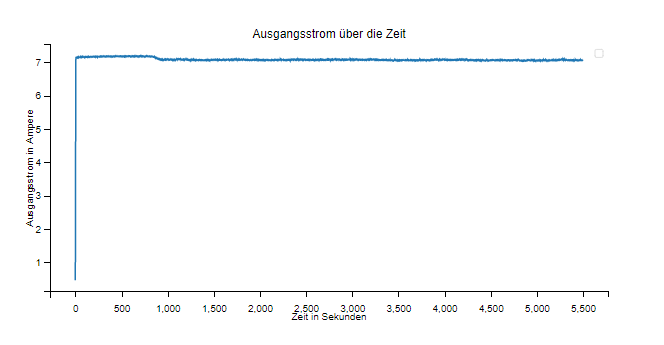
\includegraphics[height= 6cm, width = 12cm]{Pictures/B1_3P_IOUT.png}
    \caption{Ausgangsstrom über die Zeit mit Filter}
\end{figure}


\begin{figure}
    \centering
    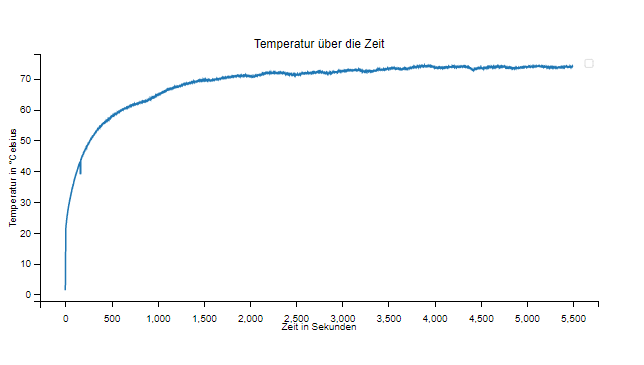
\includegraphics[height= 6cm, width = 12cm]{Pictures/B1_3P_TEMP.png}
    \caption{Temperatur über die Zeit}
\end{figure}

\begin{figure}
    \centering
    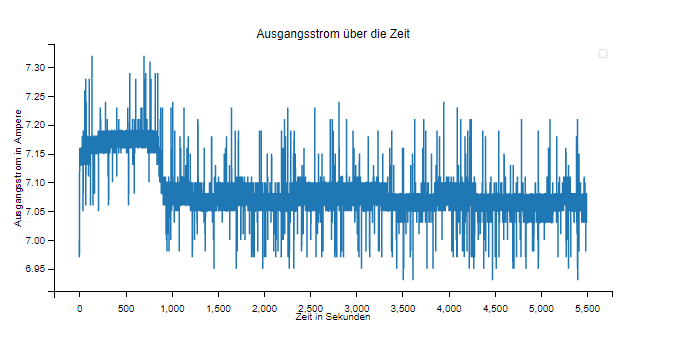
\includegraphics[height= 6cm, width = 12cm]{Pictures/B1_P3_IOUT_Rauschen.png}
    \caption{Ausgangsstrom über die Zeit}
\end{figure}

\begin{flushleft}
\hl{Bei der Temperatur ist erkenntlich, das diese anfangs Rasant ansteigt und nach etwa 1600 Sekunden auf eine Endtemperatur konvergiert. Es ist bei T = ~ 250 s erkenntlich, das der Graph einen ausreiser hat, dies hat zwei ursachen: die 1. und fundamentalste ist, dass der I2C Mikrocontroller auf dem Board in zufälligen intervallen den Wert -20.51 ausgibt, dadurch, dass dies dann entsprechend ebenfalls frequenzgefiltert wird, ergibt sich so eine kleine auslenkung}. hl{Es steht außer Frage, dass gelegentliche Sprünge zu negativen Werten, durchaus kritisch für das System sein können, wenn die Daten weiterverarbeitet und abhängig von diesen Daten Aktionen durchgeführt werden sollen. } Daher werden Daten, während sie verarbeitet werden, dahingehen überprüft, ob solche Fehlerfälle auftreten, und sofort beseitigt. \hl{Das beseitigen kann dabei mit mehreren Methoden erfolgen : }
\end{flushleft}


\begin{figure}
    \centering
    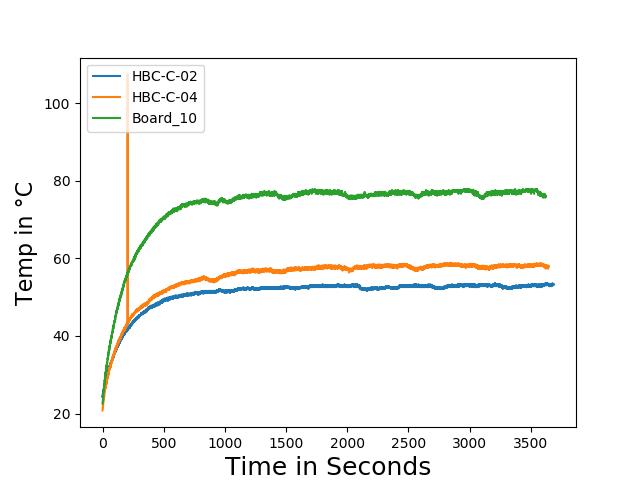
\includegraphics[height= 6cm, width = 12cm]{Pictures/3_Boards_Temp.png}
    \caption{Temperaturvergleich mehrerer Wandler}
\end{figure}


\begin{figure}
    \centering
    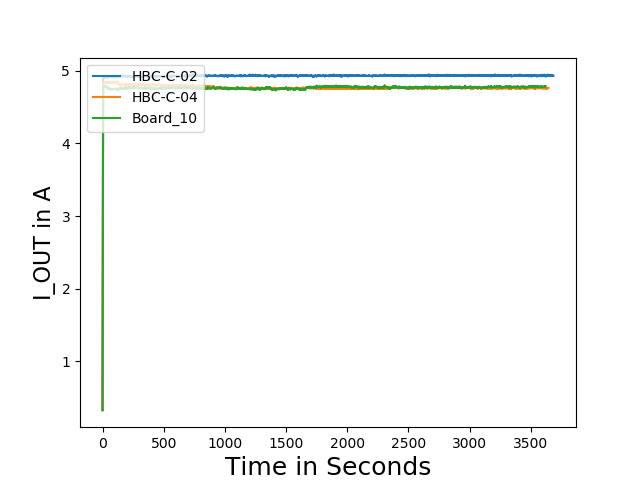
\includegraphics[height= 6cm, width = 12cm]{Pictures/Comp_IOUT.png}
    \caption{Stromvergleich mehrerer Wandler}
\end{figure}

\begin{flushleft}



Abb. 11 zeigt den gefilterten Stromverlauf der selben Wandler sowie der selben Lasten, nämlich 2 parallel geschaltene Widerstände wie in Abb. 10. Es ist zu erkennen, dass der Wandler "HB-C-02" einen höheren Strom ausgibt als die anderen beiden. Dies ist auch erkenntlich, sobald die Mittelwerte angeschaut werden: 4.933414 für HB-C-02, 4.774112 für HB-C-04 und 4.769322 für Board10. Des Weiteren ist ersichtlich, dass HB-C-04 und Board10 relativ ähnliche Ströme liefern. Ebenfalls nennenswert ist die Standardabweichung der Wandler, diese beträgt bei HB-C-02 0.0165 A, bei HB-C-04 0.0274 A und bei Board10 0.0218 A. Es zeigt sich nun, dass der Wandler HB-C-02 \hl{tendenziell besser Arbeitet als die anderen beiden, da diese geringere Schwankungen hat und höhere Ströme liefert, bzw. Ströme liefert die näher an dem theoretischen Stromfluss liegen}

In Abb. 10 ist ein Temperaturvergleich von mehreren Wandler über die Zeit dargestellt. Das offensichtlichste ist der Wandler mit der Bezeichnung "Board10", dieser hat nämlich eine über 20 Grad Celsius höhere Einschwingtemperatur. Dies ist dadurch erklärbar, dass \hl{das PWM Signal des Wandler keinen stationären Zustand erreicht}. Ein weiterer Aspekt, der sofort ersichtlich ist, ist der extreme Ausschlag beim Wandler mit der Bezeichnung "HB-C-04", bei diesem springt die Temperatur für einen kurzen Moment auf über 100 °C. Dies ist durch Fehlerhafte Sensordaten erklärbar und kann entweder nachträglich oder zur Laufzeit korrigiert werden. Eine dritte Beobachtung die gemacht werden kann, ist die, das die Wandler "HB-C-02" und "HB-C-04" relativ ähnliche Temperaturverläufe haben \hl{falls mehr Wandler verfügbar wären, könnte man die Standardabweichung und den Mittelwert präziser bestimmen}.

\hl{Diese Abbildung zeigt einen der heißesten Punkte auf dem Bord, wie der Abbildung zu entnehmen ist, zeigt sich eine Temperatur von 87° C. Dies ist eine diskrepanz von 10°C zu der maximalen Temperatur, die der Sensor aufgenommen hat. Es ist offensichtlich, dass der Sensor nicht die vollen 87° C messen kann, weil er nicht in der nahen Umgebung des Hotspots ist. Im Folgenden wird versucht die Temperaturdiskrepanz durch einführen eines Offset wertes zu minimieren, um möglichst realistische Daten zu erheben.}
\end{flushleft}